\documentclass[14pt,a4paper,oneside]{article}

\usepackage[utf8]{inputenc}   


\usepackage{amsmath,amsthm,amssymb,appendix,bm,mathrsfs,ctex,geometry,tcolorbox,fancyhdr,tikz,esint,appendix}


%% GB/T 7714 宏包 ---- 引文格式
\usepackage[sort&compress]{gbt7714}
\bibliographystyle{gbt7714-numerical}



% \numberwithin{equation}{section}             %%%%%% 公式编号




\geometry{left=1.7cm, right=1.7cm, top=2.54cm, bottom=2.54cm}    %%%%% 页面尺寸
\linespread{1.5}                             %%%%% 行距1.5倍
\pagestyle{fancy}



%%    设置页眉页脚
\fancyhf{}
\renewcommand{\headrulewidth}{0.15mm}
\fancyhead[C]{文献阅读报告}                   %%%%%% 页眉
\fancyfoot[C]{\thepage}                      %%%%%% 页脚 页码
\setlength{\headheight}{15pt}


%%   设置各种链接颜色为黑色
\usepackage[colorlinks,
            linkcolor=black,
            anchorcolor=black,
            citecolor=black,
            urlcolor=blue
            ]{hyperref}



%%   例子编号
\newcounter{example}
\counterwithin{example}{subsection}
\newcommand{\examplename}{Example}
\newcommand{\exampleTitle}[1]{%
\textbf{\refstepcounter{example}\examplename\theexample:#1}\par}


%%  插入图片配置
\usepackage{graphicx,subfigure}
\usepackage[]{caption2} %新增调用的宏包
% \numberwithin{figure}{section}               %%%%%% 图片编号按节

\graphicspath{ {./Figure/} }            %%%%% 设置图片文件所在目录
\DeclareGraphicsExtensions{.pdf,.svg,.jpeg,.png,.jpg}     %%%%% 支持图片格式


%%    支持tikz作图
\usepackage{tikz}
\usetikzlibrary{backgrounds,arrows}


\usepackage{pgfplots}
\pgfplotsset{compat=1.15}
\usepackage{mathrsfs}


\title{\textbf{文献阅读报告 12\\Nonlinear ultrafast fiber amplifiers beyond the gain-narrowing limit}\cite{sidorenkoNonlinearUltrafastFiber2019}}                           %%%%% 标题
\author{骆禹天}                                           %%%%% 作者
\date{2024/**/**}                                        %%%%%% 日期

%%   定义一些数学格式
\newtheorem{theorem}{定理}[]
\newtheorem{definition}[theorem]{定义}
\newtheorem{lemma}[theorem]{引理}
\newtheorem{corollary}[theorem]{推论}
\newtheorem{example}[theorem]{例}
\newtheorem{proposition}[theorem]{命题}
\renewcommand{\abstractname}{\Large\textbf{摘要}}




%------------------------- 开始文档  -------------------------%



\begin{document}

\pagenumbering{Roman}         %%%%% 目录前页码统计按罗马数字

\maketitle

\setcounter{page}{1}          %%%%% 标题开始统计页数

%------------------------- 目录  ------------------------------%

\tableofcontents              %%%%% 插入目录

\newpage
\setcounter{page}{1}          %%%%% 目录后重新统计页数


\pagenumbering{arabic}        %%%%% 目录后统计页码为阿拉伯数字



%%%%%%%%%%%%%%%%%%%% 开始第一节  %%%%%%%%%%%%%%%%%%%%%


\section{Introduction}

高峰值强度超快光纤激光器相较固态激光器优势:

· 紧凑性

· 良好的热光学特性

· 出色的光束质量

高峰值功率脉冲在小纤芯中长距离传播会导致大量非线性积累降低脉冲质量. 高能脉冲源通常基于啁啾脉冲放大 (CPA, 拉伸, 放大, 压缩) . 

典型 CPA 系统限制:

· 增益窄化\cite{weizhaoFemtosecondpulseFiberBased2014}

· 残余色散失配限制脉冲在 $\sim$200 fs. 

虽色散失配可通过 SPM 诱导非线性相位\cite{zhouCompensationNonlinearPhase2005}在一定程度上缓解, 但增益窄化仍然是一个持续存在的主要挑战. 

虽然 200 fs 脉冲适用于某些应用, 但其他应用（例如高次谐波产生）需要更短脉冲持续. 

解决: 

· 通过非线性压缩后续阶段获得更短脉冲 - 增加系统复杂性, 降低效率. 

· 基于非线性脉冲传播的技术, 包括直接放大\cite{zaouterStretcherfreeHighEnergy2008}和预啁啾管理\cite{liuPrechirpManagedNonlinear2015}, 以及旨在支持自相似脉冲演化的放大器\cite{andersonWavebreakingfreePulsesNonlinearoptical1993, kruglovSelfsimilarPropagationHighpower2000, fermannSelfsimilarPropagationAmplification2000}

局限性:

· 相似的放大器受益于非线性吸引子\cite{kruglovAsymptoticallyExactParabolic2006}, 该吸引子对许多种子特性没有响应, 但它们的频谱在较高能量下会溢出增益带宽, 从而降低压缩脉冲质量. 

· 使用预啁啾管理可以扩展此极限, 并达到高达微焦耳水平能量和短至 24 fs 的持续时间, 然而实现最佳性能需要精心选择种子脉冲, 因而阻碍能量扩展并增加设计的复杂性. 

\section{Result}


\subsection{Numerical Simulations}

\subsubsection{模拟概述}

图 \ref{p1} 显示典型高掺杂镱光纤放大器中的模拟脉冲演化.  

\begin{figure}[htb!]
    \centering
    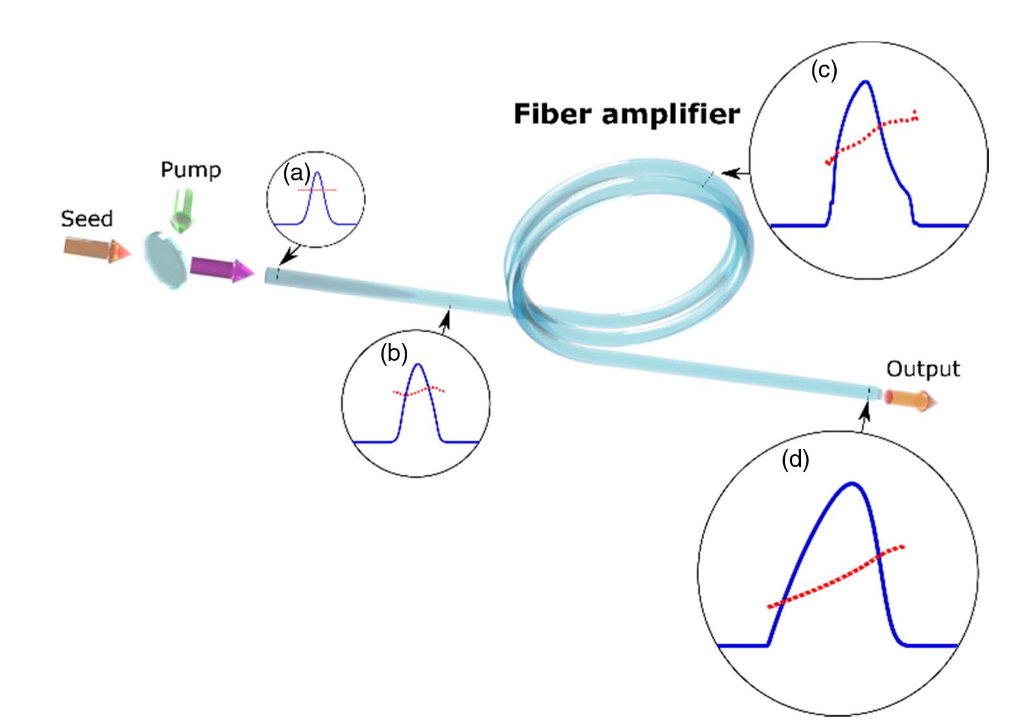
\includegraphics[width=0.5\textwidth]{p1.png}
    \caption{GMN 放大机制的模拟示例}\label{p1}
\end{figure}

· 1028 nm 的 0.5 nJ, 0.8 ps 高斯脉冲输入

纤芯直径 6 $\mathrm{\mu m}$ 双包层掺镱光纤放大器

· 976 nm 处进行共泵浦. 

数值模型:

· 二阶和三阶色散效应, 

· SPM, 自陡峭, 拉曼散射

· 通过与脉冲演化同时求解粒子数反转率方程计算的增益\cite{denbaarsGuestEditorialIntroduction2022, lindbergAccurateModelingHighrepetition2016}. 

脉冲演化:

· 最初遵循众所周知的轨迹：色散效应和非线性效应都很普遍, 迅速演化为自相似脉冲或相似脉冲\cite{kruglovSelfsimilarPropagationHighpower2000, fermannSelfsimilarPropagationAmplification2000}[图\ref{p1} (b)]. 

· 随着脉冲能量和带宽的增加, 增益整形开始阻碍相似性的增长, 导致预期的非线性脉冲失真和自相似传播的损失\cite{sohEfficientFemtosecondPulse2006, peacockSolitaryPulsePropagation2002}[图\ref{p1} (c)]. 

· 传统上, 这一点被认为是自相似放大的极限. 然而如果允许脉冲演化继续, 就会出现新的状态. 随着反转的衰减, 脉冲向更长的波长移动, 并在光谱和时间域中继续展宽. 脉冲能量增加, 脉冲演变为不对称的时间分布[图\ref{p1} (d)]. 

· 新脉冲产生了单调的线性调频脉冲, 可通过光栅对补偿.

作者指出: 为了了解这种超出自相似放大范围的新机制的起源, 对根据速率方程计算出的真实增益进行建模, 从而进行额外更详细模拟至关重要. 

因为掺镱光纤的准三能级性质导致增益谱随着泵浦光和信号光的不同分量被吸收和重新发射而动态变化. 这导致纵向演变的增益谱以及非线性和增益整形的作用相互交织, 最终实现非线性相位的管理并维持可压缩的频率啁啾. 

GMN 放大主要特征如图 \ref{p2} 和图 \ref{p3} 所示. 当种子波长选择接近光纤中吸收和增益之间的转变时, 信号和增益的相互作用可以在高掺杂的光纤中得到增强. 因此作者保持与以前相同的 1028 nm 种子波长, 但将变换限制持续时间增加到 2 ps, 以探索不同种子脉冲的使用. 

\subsubsection{GMN中脉冲演变 (时域和频域)}

\begin{figure}[htb!]
    \centering
    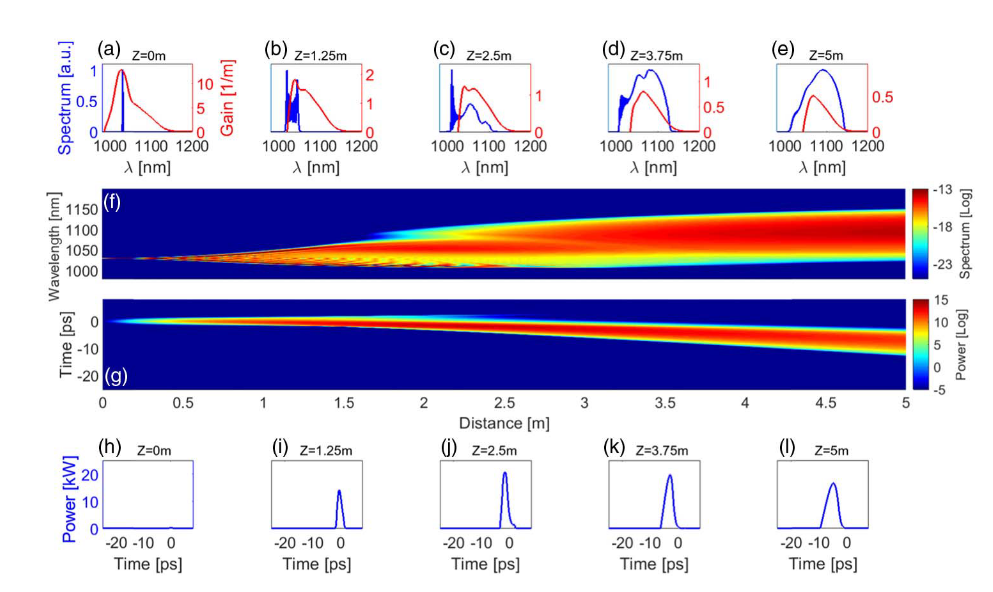
\includegraphics[width=0.7\textwidth]{p2.png}
    \caption{掺镱光纤中脉冲演化模拟. 顶部两行 [(a)-(f)] 显示放大脉冲的频谱演变（蓝色）和饱和增益频谱（红色）, 而底部两行 [(g)-(l)] 显示脉冲的时间进化. } \label{p2}
\end{figure}

最初, 脉冲演化由 SPM 主导 [图\ref{p2}(a)和(b)]:

· 值得注意, 在$\sim$ 2 m 后脉冲开始朝平滑、不对称的时间形状演化, 而不是经历预期的破波扭曲\cite{feijooperezNewAspectsMatter2016, nelsonLargeNonlinearPulse1983}.  

增益谱的纵向演变如图 2(a)-2(e) 带有红色实线:

当非线性频谱展宽平衡增益整形时, 可以实现 \textbf{GMN 机制}. 这种平衡表现为光谱蓝色部分的吸收和红色部分的放大 [图 \ref{p2}(c)-\ref{p2}(e)、\ref{p1}(j)-\ref{p2} 和 \ref{p3}(a)]. 

尽管与传统放大器设计规则背道而驰, 但在脉冲放大过程中有意使用增益和损耗是 GMN 机制的一个重要方面. 

\begin{figure}[htb!]
    \centering
    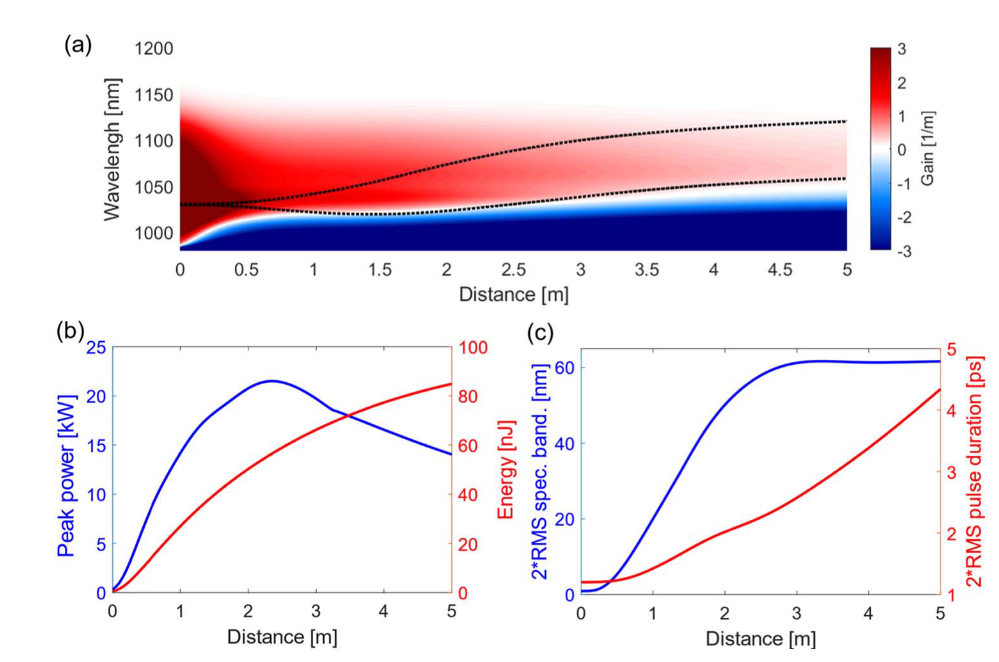
\includegraphics[width=0.6\textwidth]{p3.png}
    \caption{GMN 放大器中的脉冲和增益演变: (a) 增益谱纵向演变, 黑色虚线标记光谱（中心波长即均方根带宽）; (b) 峰值功率（蓝色）和脉冲能量（红色）与传播距离关系.  (c) 脉冲的带宽（蓝色）和啁啾持续时间（红色）与传播距离关系. }\label{p3}
\end{figure}

\subsubsection{增益与色散间动态平衡}

此外, 与所有其他放大机制不同, 脉冲峰值功率不会随通过放大器的传播而单调增加. 相反它在 $\sim$ 2 m 处达最大, 此后逐渐减小 [图 \ref{p2}(h)-\ref{p2}(l) 和 \ref{p3}(b)]. 这种非单调行为是由于增益和色散之间的动态平衡造成的, 如图 \ref{p3}(b)和\ref{p3}(c). 

在演化的初始阶段, 脉冲向抛物线吸引子演化, 由于接近指数的宽带（相对于脉冲）增益, 峰值功率按预期增长, 并且脉冲带宽增加. 由于非线性增加的带宽, 色散的影响会增加, 而放大率会随着更多的泵浦被吸收而降低；

传播约 2 m 后, 色散时间展宽克服了增益并导致峰值功率随后下降. 在持续时间增加的帮助下, 脉冲能量继续单调增加, 同时脉冲保持其时域强度分布. 

密切比较脉冲和增益的频谱演变有助于了解 GMN 状态. 

· 当光谱的蓝色一侧遇到 1020 nm 附近的吸收时, 初始光谱展宽被抑制[图 \ref{p3}(a)]. 

· 随着不断演化, 这种吸收特征和增益窗口都会转向红色, 因此脉冲光谱的蓝色一侧受到限制, 而其红色一侧继续不受阻碍地变宽. 

· 随着峰值功率和净增益开始衰减, 脉冲光谱带宽的增长饱和, 受到蓝色侧残留吸收和红色侧增益消失的限制. 这是放大器输出端出现的不对称稳态脉冲的起源[图 \ref{p2}(f)和\ref{p4}(a)]. 

\subsubsection{易压缩}

令人惊讶的是, 在这种复杂且动态的光谱成分混合之后, 脉冲[图\ref{p4}(a)]可以很容易地压缩到接近变换极限[图\ref{p4} (b)]. 光栅压缩器的标准设计很容易适应线性调频脉冲的偏差. 因此, 尽管存在极其非线性和宽带脉冲演化, 但简单的光栅压缩器足以产生高质量、几乎变换受限的脉冲. 

尽管有 120 $\pi$ 的非线性相位累积, 但这种压缩的清洁度是相似演化的标志；然而, 脉冲在其传播轨迹、带宽和整体性能方面显然已超出了自相似. 当从计算中消除高阶色散和自陡峭时, GMN 脉冲演化保持不变. 因此, 它只需要群速度色散、SPM 和根据速率方程计算的真实增益. 

\subsubsection{非线性吸引子的数值证据}

\begin{figure}[htb!]
    \centering
    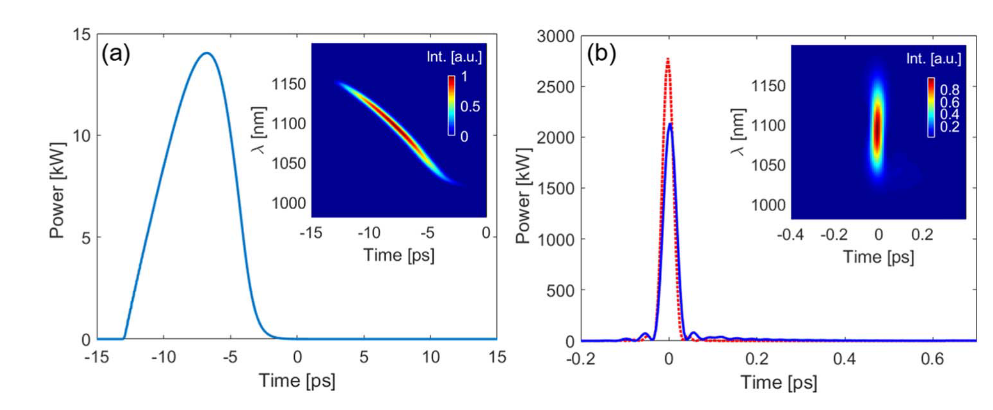
\includegraphics[width=0.6\textwidth]{p4.png}
    \caption{GMN 放大生成脉冲: (a) 图 \ref{p2} 示例中线性调频输出脉冲. (b) 压缩脉冲（蓝色实线）和变换限制脉冲（红色虚线）.  (a) 和 (b) 中的插图分别显示了线性调频脉冲（由 1-ps 高斯窗口选通）和压缩脉冲（由 5-fs 高斯窗口选通）的频谱图. }\label{p4}
\end{figure}

模拟还表明最终的不对称脉冲形状是非线性吸引子. 亦即, GMN 中脉冲演化更多由非线性和增益整形驱动的, 而不是由种子脉冲的特定参数驱动的. 

为了证明这一点, 作者模拟发射跨越一系列形状、能量、持续时间、线性调频、带宽和峰值功率的种子脉冲[图\ref{p5}(a)]进入固定放大器. 

不同的脉冲以类似的方式演化：每个脉冲在进入 GMN 放大区域之前都会经历一个初始的、SPM 主导的瞬态. 

这两种状态之间的转变取决于种子脉冲, 并且可以根据峰值功率进行近似, 峰值功率在转变点附近达到最大值, 然后随着 GMN 状态的特征而减小[图 \ref{p5}(b)]. 特别是, 尽管不同脉冲以不同速率演化, 但可通过记录每个脉冲在何处跨越峰值功率阈值[图 \ref{p5}(b) 中的黑色虚线], 在演化中的等效点对它们进行比较. 

此时, 脉冲几乎相同 [图 \ref{p5}(c)], 提供了强有力的证据证明放大的脉冲是非线性吸引子. 

\begin{figure}[htb!]
    \centering
    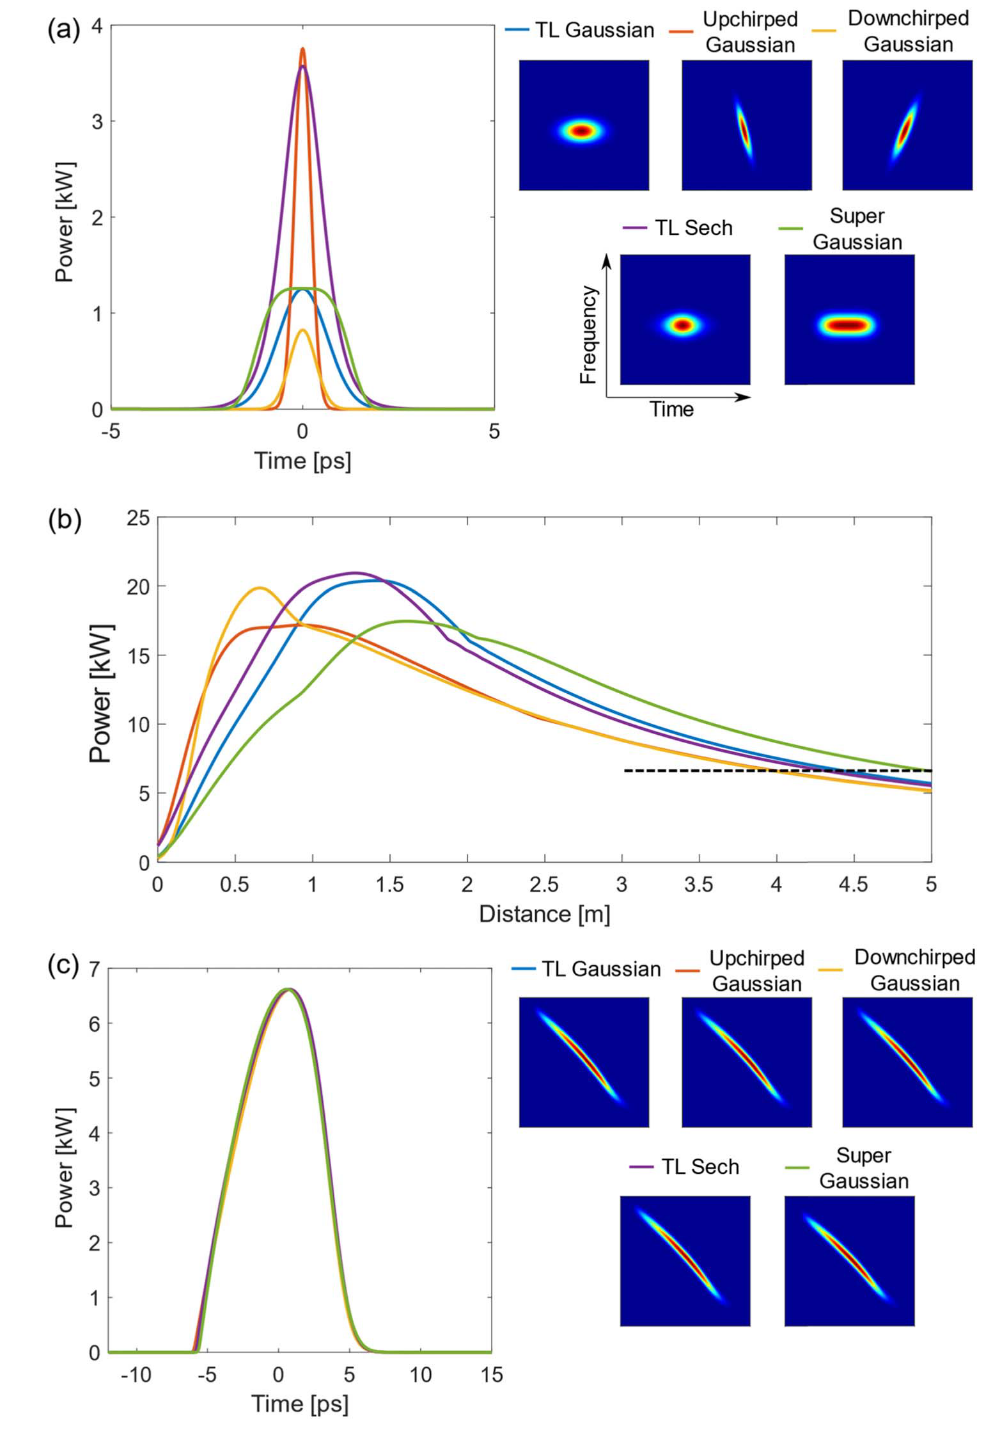
\includegraphics[width=0.5\textwidth]{p5.png}
    \caption{非线性吸引子的数值证据.  (a) 不同的种子脉冲及其相应的频谱图.  TL：变换受限.  (b) 每个种子的峰值功率的演变.  (c) 在相同功率水平下使用不同种子产生的放大脉冲[由(b)中的黑色虚线表示, 任意选择为 6.6 kW]. }\label{p5}
\end{figure}

\subsubsection{非线性吸引子与自相似对比分析}

据作者所知, 正常色散放大器中唯一的其他非线性吸引子是相似的\cite{kruglovSelfsimilarPropagationHighpower2000, fermannSelfsimilarPropagationAmplification2000}. 相似性和 GMN 体系是否可能相关? 目前作者认为并非如此. 

区分:

1. 众所周知, 虽然自相似可以存在于各种均匀加宽\cite{kruglovSelfsimilarPropagationHighpower2000}和饱和\cite{kruglovParabolicHypergaussianSimilaritons2012}增益模型中, 但它们在存在增益整形的情况下会失真并变得不可压缩\cite{sohEfficientFemtosecondPulse2006, peacockSolitaryPulsePropagation2002}. 相比之下, GMN 机制只有在存在强烈的增益整形（包括增益和损失的影响）时才能存在. 图 \ref{p2} 中的频谱说明了这一点, 该频谱在脉冲传播大部分时间里明显超出了增益带宽 [图 \ref{p2}(a)-(e)的红色曲线]. 

2. 自相似的特点是能量、持续时间、峰值功率和带宽呈指数增长.  GMN 体系中的脉冲仅在持续时间内增长 [图 \ref{p3}(c)], 而其能量和带宽饱和[图 \ref{p3}(b)和(c)]并且其峰值功率降低[图\ref{p3}(b)]. 然而, 对 GMN 机制性质的进一步研究可能会揭示这两个吸引子背后的联系. 

\subsection{Experimental Results}

· 5 m, 芯直径 5 $\mathrm{\mu m}$ 高掺杂双包层 Yb 光纤 (Nufern PM-YDF-5/130-VIII) 中 GMN 放大, 976 nm 二极管共同泵浦. 

· 输入放大器: 变换极限的 700-fs、1-nJ 脉冲, 脉冲通过对全法向色散飞秒光纤激光器压缩输出的蓝色部分进行光谱过滤生成\cite{chongAllnormaldispersionFemtosecondFiber2007}. 

· 种子的重复率: 12.5 MHz. 

\subsubsection{GMN放大表征}

\begin{figure}[htb!]
    \centering
    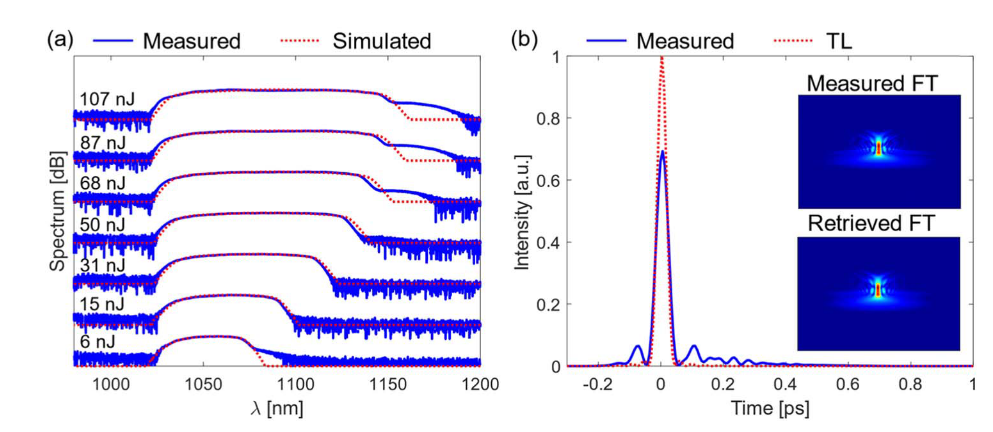
\includegraphics[width=0.6\textwidth]{p6.png}
    \caption{GMN 放大器实验: (a) 增加泵浦功率时测量（蓝色实线）和模拟（红色虚线）输出光谱; (b) 压缩（蓝色实线）107 nJ 脉冲和变换限制脉冲（红色虚线）; (b) 中的插图显示了测量和检索的 SHG-FROG 迹线。}\label{p6}
\end{figure}

· 随泵浦功率增加, 光谱显着变宽, 与模拟一致[图 \ref{p6}(a)]. 测得带宽迅速增长到超 1100 nm, 溢出了掺镱增益介质的带宽. 

· 用光栅压缩器能将放大脉冲压缩至变换极限, 这表明生成带宽是相干的, 而非源自散粒噪声种子拉曼散射. 使用色散傅立叶变换测量\cite{tongFibreDispersionPulse1997}（未显示）进一步证实了脉冲在整个带宽上的相干性, 这表明单次脉冲光谱稳定且低噪声. 

· 对于 68 nJ 或更高的脉冲能量, 可观察到拉曼散射, 但仅作为可与主脉冲清晰区分的低强度光谱肩. 在最高输出脉冲能量（107 nJ, 其中拉曼贡献小于脉冲能量的 3\%）时, 放大的脉冲被压缩至 42 fs, 接近变换极限 [图 \ref{p6}(b)]. 可注意到 89\% 的能量位于主脉冲中, 只有 11\% 的能量分布在未压缩的基座中.  （补充 1 的图 S1 讨论了模拟斯托克斯波和实验斯托克斯波之间的定量差异. ）

\begin{figure}[htb!]
    \centering
    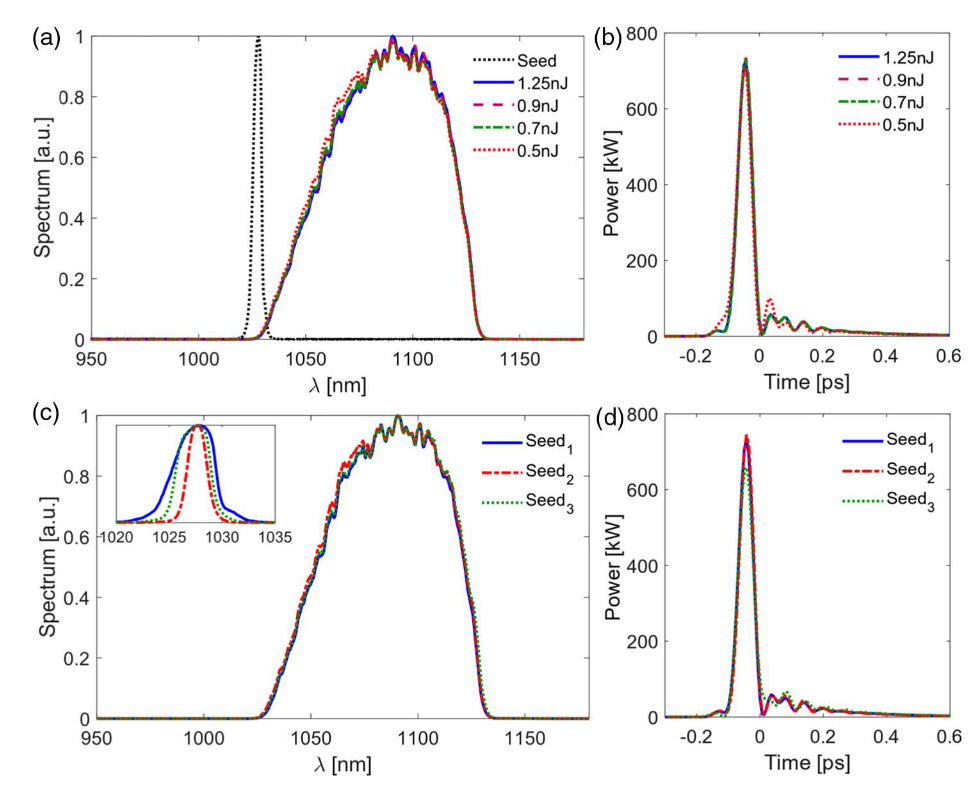
\includegraphics[width=0.6\textwidth]{p7.png}
    \caption{非线性吸引子实验证据: (a) GMN 放大器的输出频谱和 (b) 恒定种子频谱的相应压缩脉冲 [(a) 中的黑色虚线]，具有指示的种子脉冲能量。 (c) 以恒定种子能量作为种子的 GMN 放大器的输出频谱和脉冲形状（插图：种子频谱），以及 (d) 相应的去线性调频脉冲。}\label{p7}
\end{figure}

\subsubsection{非线性吸引子}

为了研究脉冲演化为非线性吸引子的数值预测, 作者向放大器发射各种种子脉冲. 

· 一项实验中, 种子光谱和持续时间保持恒定, 而能量变化近 3 倍 [图 \ref{p7}(a)和7(b)]; 

· 另一实验中, 用滤波器改变变换极限种子带宽（从而改变其持续时间）, 同时其能量保持恒定在 0.5 nJ [图 \ref{p7}(c)和(d)]. \textbf{无论哪种类型的变化, 输出频谱 [图 \ref{p7}(a) 和 (c)] 和压缩脉冲 [图 \ref{p7}(a)和7(c)] 和压缩脉冲 [图 \ref{p7}（b）和（d）] 几乎保持不变, 尤其其中并没有调整泵浦功率或光栅压缩器}. 

· 这种输出脉冲对输入种子特性的明显的不敏感性强烈表明非线性吸引子是 GMN 放大机制的基础. 

\subsubsection{吸引脉冲形状}

\begin{figure}[htb!]
    \centering
    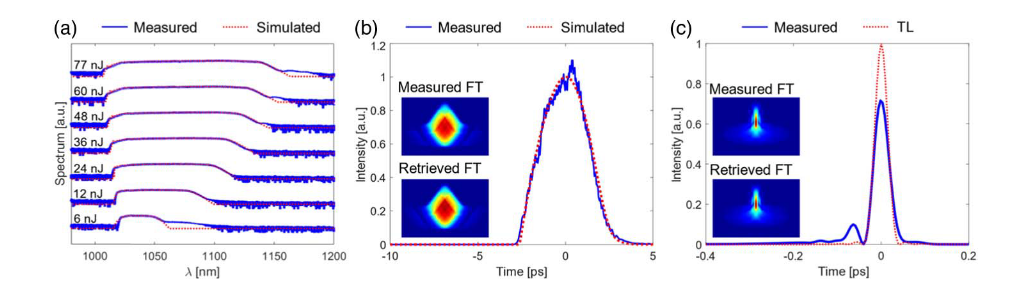
\includegraphics[width=0.7\textwidth]{p8.png}
    \caption{直接测量 GMN 放大器啁啾脉冲: (a) 增加泵浦功率时的测量光谱（蓝色实线）和模拟光谱（红色虚线）; (b) 与 (a) 中的 77-nJ 结果相对应的测量（蓝色实线）和模拟（红色虚线）脉冲形状; (c) 测量的压缩脉冲（蓝色实线）和计算的变换限制脉冲（红色虚线）。}\label{p8}
\end{figure}

考虑到 GMN 区域中吸引脉冲形状的重要性, 直接从放大器测量脉冲并将其与仿真进行比较非常重要.

不幸频率分辨光门控（FROG）仪器缺乏测量上述放大器的啁啾脉冲的扫描范围. 

因此, 作者构建了一个较短的放大器, 由能量为 3 nJ 的窄带变换限制脉冲作为种子. 这会产生更短、能量更低、带宽更低的放大脉冲, 可以直接使用 FROG 进行测量. 

· 该放大器仿真与测量结果吻合良好（图 \ref{p8}）. 

· 作者将脉冲能量限制为 77 nJ 以限制带宽. 

· 测量的输出脉冲表现出预期不对称时间形状, 且与模拟非常吻合[图 \ref{p8}(b)], 并且可以被压缩到接近变换极限[图 \ref{p8}(c)]. 

\section{Discussion}

· 研究 GMN 体系中的脉冲能量缩放到大模场面积 (LMA) 光纤也将很有趣：对于双包层 LMA 光纤，泵浦吸收速率将以非平凡的方式影响纵向增益演化，这可能会影响纵向增益的演化。导致缩放关系比简单的模式区域缩放更复杂。

· 其他广泛使用的增益介质，例如掺铒、掺铥和掺钕光纤;

· 研究可控增益与损失的系统;

· 由 NLSE 与速率方程的理论解释;

应用: 

· 可以减少或补偿种子脉冲源中的噪声或漂移;

· 结合 GMN 光纤放大器与大芯、高度多模光纤, 不牺牲光束质量


%--------------------  插入参考文献  --------------------%

\newpage

\clearpage           %%%  “目录”中显示的页码正确, 需要添加 \clearpage
\phantomsection      %%   “目录”中的链接能正确跳转, 需要添加 \phantomsection
\addcontentsline{toc}{section}{参考文献}   %向目录中添加条目, 以章的名义

\bibliography{ref}

\end{document}